\documentclass[entwurf.tex]{subfiles}

\begin{document}

\chapter{Sequenzdiagramme}
	\section{Terminal connect}
		In dem folgenden Diagramm sieht man den Ablauf vom Verbinden eines Endgeräts mit dem Server bis zur Live-Übertragung der Signale und die Änderung der Anzeigekonfiguration auf dem Endgerät. 
		\begin{figure}[H]
 			\makebox[\textwidth][c]{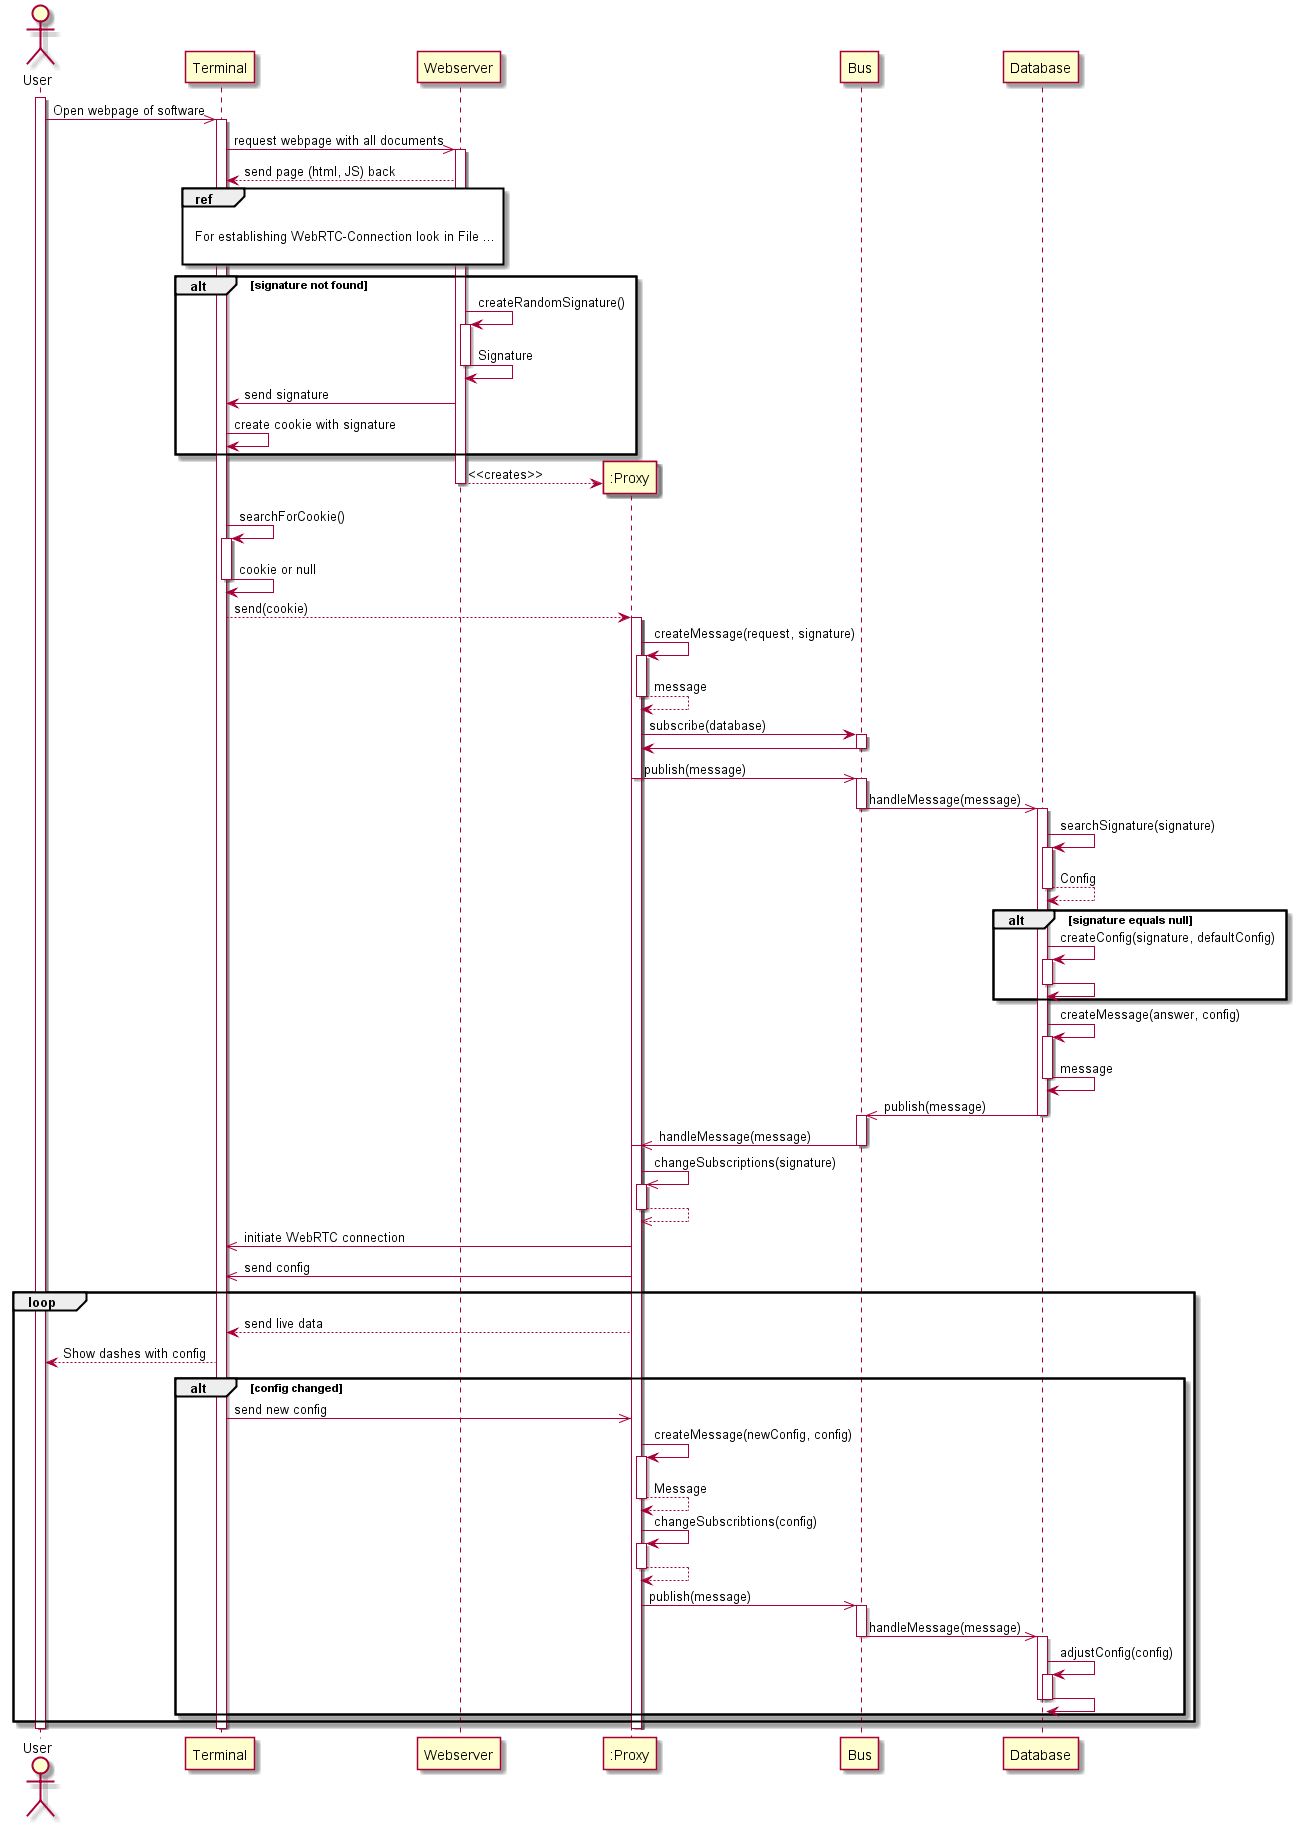
\includegraphics[width=0.9\paperwidth]{diagrams/Connect.png}}
  			\caption{Verschiedene Dash-Anzeigeelemente.}
  		\end{figure}
	\section{Parkingsensor}
		Der Ablauf beim Start des Parksensors
		\begin{figure}[H]
  			\begin{center}
 				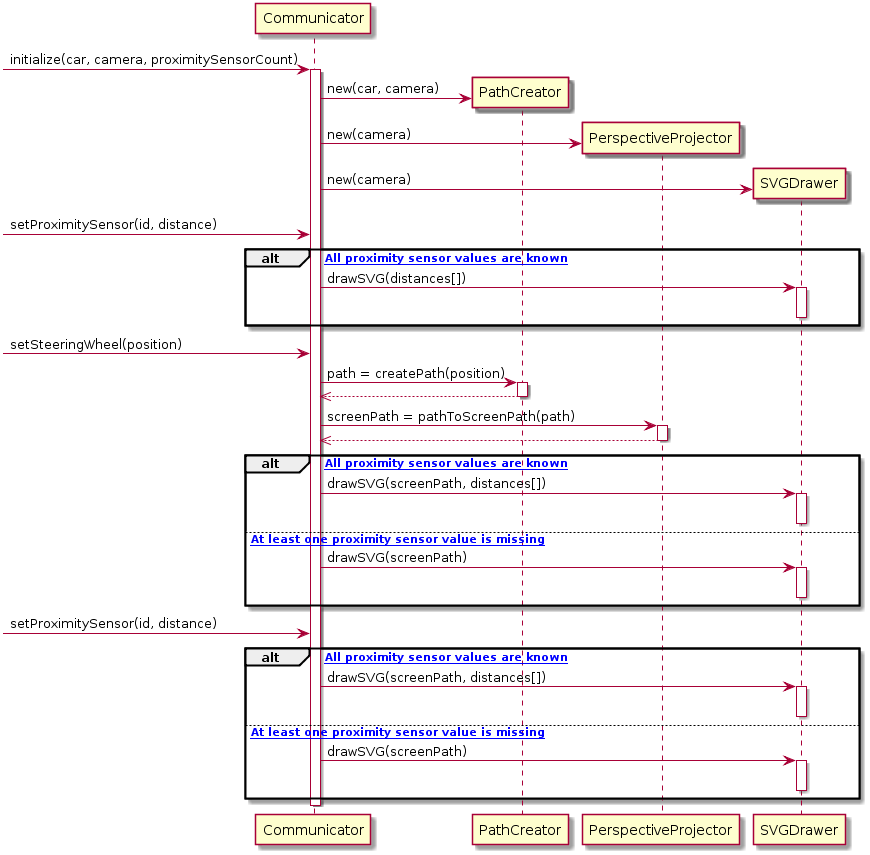
\includegraphics[width=\textwidth]{diagrams/ParkingSensor/sequence_diagram.png}
  				\caption{Verschiedene Dash-Anzeigeelemente.}
  			\end{center}
  		\end{figure}
\end{document}